\documentclass{sigchi}

% Use this command to override the default ACM copyright statement
% (e.g. for preprints).  Consult the conference website for the
% camera-ready copyright statement.


%% EXAMPLE BEGIN -- HOW TO OVERRIDE THE DEFAULT COPYRIGHT STRIP -- (July 22, 2013 - Paul Baumann)
% \toappear{Permission to make digital or hard copies of all or part of this work for personal or classroom use is      granted without fee provided that copies are not made or distributed for profit or commercial advantage and that copies bear this notice and the full citation on the first page. Copyrights for components of this work owned by others than ACM must be honored. Abstracting with credit is permitted. To copy otherwise, or republish, to post on servers or to redistribute to lists, requires prior specific permission and/or a fee. Request permissions from permissions@acm.org. \\
% {\emph{CHI'14}}, April 26--May 1, 2014, Toronto, Canada. \\
% Copyright \copyright~2014 ACM ISBN/14/04...\$15.00. \\
% DOI string from ACM form confirmation}
%% EXAMPLE END -- HOW TO OVERRIDE THE DEFAULT COPYRIGHT STRIP -- (July 22, 2013 - Paul Baumann)


% Arabic page numbers for submission.  Remove this line to eliminate
% page numbers for the camera ready copy 

%\pagenumbering{arabic}

% Load basic packages
\usepackage{balance}  % to better equalize the last page
\usepackage{graphics} % for EPS, load graphicx instead 
%\usepackage[T1]{fontenc}
\usepackage{txfonts}
\usepackage{times}    % comment if you want LaTeX's default font
\usepackage[pdftex]{hyperref}
% \usepackage{url}      % llt: nicely formatted URLs
\usepackage{color}
\usepackage{textcomp}
\usepackage{booktabs}
\usepackage{ccicons}
\usepackage{todonotes}
\usepackage{multirow}

% llt: Define a global style for URLs, rather that the default one
\makeatletter
\def\url@leostyle{%
  \@ifundefined{selectfont}{\def\UrlFont{\sf}}{\def\UrlFont{\small\bf\ttfamily}}}
\makeatother
\urlstyle{leo}

% To make various LaTeX processors do the right thing with page size.
\def\pprw{8.5in}
\def\pprh{11in}
\special{papersize=\pprw,\pprh}
\setlength{\paperwidth}{\pprw}
\setlength{\paperheight}{\pprh}
\setlength{\pdfpagewidth}{\pprw}
\setlength{\pdfpageheight}{\pprh}

% Make sure hyperref comes last of your loaded packages, to give it a
% fighting chance of not being over-written, since its job is to
% redefine many LaTeX commands.
\definecolor{linkColor}{RGB}{6,125,233}
\hypersetup{%
  pdftitle={SIGCHI Conference Proceedings Format},
  pdfauthor={LaTeX},
  pdfkeywords={SIGCHI, proceedings, archival format},
  bookmarksnumbered,
  pdfstartview={FitH},
  colorlinks,
  citecolor=black,
  filecolor=black,
  linkcolor=black,
  urlcolor=linkColor,
  breaklinks=true,
}

% create a shortcut to typeset table headings
% \newcommand\tabhead[1]{\small\textbf{#1}}

% End of preamble. Here it comes the document.
\begin{document}

\title{Finding Bottlenecks: Predicting Student Attrition with Unsupervised Classifiers}

\numberofauthors{5}
\author{%
  \alignauthor{Christopher McKinlay\\
    \affaddr{California State University, Northridge}\\
    \affaddr{Northridge, USA}\\
    \email{chris.mckinlay@gmail.com}}\\
 \alignauthor{Efunwande Osoba\\
    \affaddr{California State University, Northridge}\\
    \affaddr{Northridge, USA}\\
    \email{eosoba@gmail.com}}\\
  \alignauthor{Allen Sarkisyan\\
    \affaddr{California State University, Northridge}\\
    \affaddr{Northridge, USA}\\
    \email{programminglinguist@gmail.com}}\\
  \alignauthor{Seyed Sajjadi\\
    \affaddr{California State University, Northridge}\\
    \affaddr{Northridge, USA}\\
    \email{Seyed Sajjadi.947@my.csun.eud}}\\
  \alignauthor{Carol Shubin\\
    \affaddr{California State University, Northridge}\\
    \affaddr{Northridge, USA}\\
    \email{carol.shubin@csun.edu}}\\
}

\maketitle
\begin{abstract}
  
With pressure to increase graduation and reduce time to degree in higher education, it is important to identify at-risk students early. Automated early warning systems are therefore highly desirable. In this paper, we use unsupervised clustering techniques to predict the graduation status of declared majors in four departments at California State University Northridge (CSUN), based on a minimal number of lower division courses in each major. In addition, we use the detected clusters to identify hidden bottleneck courses. 
\end{abstract}

\keywords{educational data\-mining; clustering; regression; k\-means}

\category{H.5.m.}{Information Interfaces and Presentation
  (e.g. HCI)}{Miscellaneous} 
\category{K.3.1.}{Computer Uses in Education }{}


\section{INTRODUCTION}

Policy makers, the public, university administrators, students and their families are concerned about low graduation rates and lengthy times to degree in higher education. At CSUN for example, the median time to degree is six years and the six-year graduation rate is 41\% ~\cite{csun1}. A related issue is the incidence of major-switching, since re-declaring a major is time-consuming and costly. Approximately 24\% of CSUN students re-declare their major, and the plurality of these changes involve departments in the David Nazarian College of Business and Economics (CoBaE) ~\cite{csun2}. For this reason we focused our analysis on four departments within the CoBaE.

With an enrollment of over 6000 undergraduate students, CoBaE is one of largest business schools in the nation. CoBaE confers the second most undergraduate degrees at CSUN (behind the College of Social and Behavioral Science), and it has three of the top ten most popular majors (management, finance, and marketing) at CSUN. 

In this paper, we trained K-means classifiers on grade data from undergraduate majors in the CoBaE: economics, business law, management, and marketing. Strongly predictive clusters were present in each of the four departments. We found that cluster separation was driven disproportionately by a small number of bottleneck courses. We also found that training classifiers on just the first three classes on the graduation pathway was an effective early detection method. 









\section{RELATED WORK}

Educational data mining is an emerging discipline, concerned with developing methods for exploring the unique types of data that come from the educational sphere. The field encompasses various subdomains such as modeling student learning to better optimize performance, to detecting outliers, to developing automated tutoring systems that intelligently adapt lesson plans to the individual learning styles, see ~\cite{romero2010educational}. 

Luan ~\cite{luan2002data} studied clustering aspect of data mining offers comprehensive characteristics analysis of students and offered likelihood estimates for a variety of outcomes, such as transferability, persistence, retention, and success in classes.  Al-Radaideh et al. ~\cite{al2006mining} applied classification techniques to determine the main attributes that may affect student performance. Tair and El-Halees ~\cite{tair2012mining}, used K-means to predict graduate students’ performance, and overcome the problem of low grades of graduate students.  Ayesha, Mustafa, Sattar and Khan ~\cite{ayesha2010data} have also used K-means clustering to predict student performance in a particular course. Romero, Ventura and García ~\cite{romero2008data} described the full process of clustering, classification, statistics and visualization in the context of mining Moodle (e-learning) data. Our current work uses unsupervised clustering methods to address the issue of large scale student behavior.









\section{METHOD}

\subsection{Data Collection and Preprocessing}

We obtained academic records containing grade information from declared majors in four departments in the College of Business and Economics at CSUN. The majors we inspected were Economics, Management, Marketing and Business Law. The data spans a fifteen year period between 2000 and 2014—containing 13,484 student records in total—and contains only the courses required for each major. 

The grade data for each course were encoded with the following normalized GPA scale prior to statistical analysis: 

\begin{table}[h]
\scalebox{0.8}{
\begin{tabular}{llllllllllll}
A   & A-  & B+  & B   & B-  & C+  & C & C-   & D+   & D    & D-   & F \\
2.0 & 1.7 & 1.3 & 1.0 & 0.7 & 0.3 & 0.0 & -0.3 & -0.7 & -1.0 & -1.3 &  -2.0
\end{tabular}}
\caption{Grade encoding scheme}~\label{tab:gradeEncodingTable}
\end{table}

Missing data was encoded as an ‘F’ in order to facilitate the analysis, since not taking a required course has the same effect as failing it. The datasets were separated by majors, with columns for graduation, number of semesters in the major, number of credits for the major, followed by the course names. 


\subsection{Cluster Analysis}

There are a few fundamental issues involved in cluster analysis, notably determining whether discrete clusters are present ~\cite{knights2014rethinking} and choosing the appropriate number of clusters ~\cite{gordon1999classification} ~\cite{duda2012pattern}. We applied the K-means algorithm ~\cite{macqueen1967some} to the grade data and used the Calinski-Harabasz (CH) index \cite{calinski1974dendrite} to determine the optimal number of clusters on fivefold cross-validated datasets (\ref{fig:CHindex}).

We then established the predictive power of the clusters by testing them on a classification task. We compared the cluster-based classifiers with logistic regression classifiers in predicting the graduation status of hold-out samples for each department. Receiver Operating Characteristic (ROC) curves were then used to evaluate and compare predictive performance of clustering and logistic regression methods for each department (\ref{tab:rocTable}). Finally, we performed the same steps to predict graduation status based on the typical first three courses in each major.


\section{RESULTS}

The optimal number of clusters was determined to be two in all departments (see \ref{fig:CHindex}). The Management and Marketing departments showed better between-cluster separation than Economics and Business Law. 

We applied the same approach to the first three classes that students would normally take within their first year at school. Table \ref{tab:scoresTable} shows the Accuracy, Precision, Recall, F1 Scores and False Omission Rates resulting from the both classifiers when trained on the full feature set and on the first three courses in each major. 


% Please add the following required packages to your document preamble:
% \usepackage{multirow}
\begin{table}[h]
\scalebox{0.6}{
\begin{tabular}{ccccccc}
                                                                         & Model & Accuracy & Precision & Recall & F1 Score & False Omission Rate\\
\multirow{4}{*}{Management}                           & Logistic Full Set & 0.91 & 0.82 & 0.91 & 0.86 & 0.04
     \\
                                                                         & Logistic 3 Courses & 0.7 & 0.48 & 0.31 & 0.38 & 0.25
     \\
                                                                         & KMeans Full Set & 0.78 & 0.57 & 1.0 & 0.73 & 0.0
     \\
                                                                         & KMeans 3 Courses & 0.65 & 0.46 & 0.88 & 0.6 & 0.08
    \\

\multirow{4}{*}{Economics}                              & Logistic Full Set & 0.86 & 0.81 & 0.83 & 0.82 & 0.1
  \\
                                                                         & Logistic 3 Courses & 0.64 & 0.54 & 0.45 & 0.49 & 0.32
    \\
                                                                         & KMeans Full Set & 0.82 & 0.7 & 0.94 & 0.8 & 0.05
     \\
                                                                         & KMeans 3 Courses & 0.45 & 0.21 & 0.16 & 0.18 & 0.46
    \\

\multirow{4}{*}{Marketing}                                & Logistic Full Set & 0.88 & 0.8 & 0.89 & 0.84 & 0.06
     \\
                                                                         & Logistic 3 Courses & 0.68 & 0.54 & 0.51 & 0.52 & 0.25
     \\
                                                                         & KMeans Full Set & 0.78 & 0.63 & 0.99 & 0.77 & 0.0
     \\
                                                                         & KMeans 3 Courses & 0.78 & 0.63 & 0.99 & 0.77 & 0.0
     \\
\multirow{4}{*}{\begin{tabular}[c]{@{}c@{}}Business \\ Law\end{tabular}} & Logistic Full Set & 0.79 & 0.72 & 0.69 & 0.71 & 0.17
     \\
                                                                         & Logistic 3 Courses & 0.63 & 0.5 & 0.38 & 0.43 & 0.32
     \\
                                                                         & KMeans Full Set & 0.73 & 0.58 & 0.96 & 0.72 & 0.04
     \\
                                                                         & KMeans 3 Courses & 0.73 & 0.58 & 0.96 & 0.72 & 0.04
    
\end{tabular}}
\caption{Accuracy, Precision, Recall, F1 Scores, and the False Omission Rate}~\label{tab:scoresTable}

\end{table}

We expected that a predictive model trained on the full feature set of course grades would be more effective than a model using cluster labels from unsupervised clustering. To test this hypothesis, we compared the performance of a logistic regression classifier trained on the full feature set to the performance of a classifier that used co-membership information from the clusters on a classification task: to predict whether the student had in fact graduated with that major. The cluster-based classifier estimated the probability that a student belonged to a particular category using the fraction of co-clustered samples that also belonged to the category of interest.

In each case we identified strongly predictive clusters. Though outperformed, the cluster-based classifiers compared surprisingly well with the logistic regression models (see \ref{tab:rocTable}). Heuristically speaking, students in the same cluster tended to drop out at the same times after getting the same grades in the same courses. 

\begin{table}[ht]
 \begin{center}
   \begin{tabular}{ c }
   \hline
   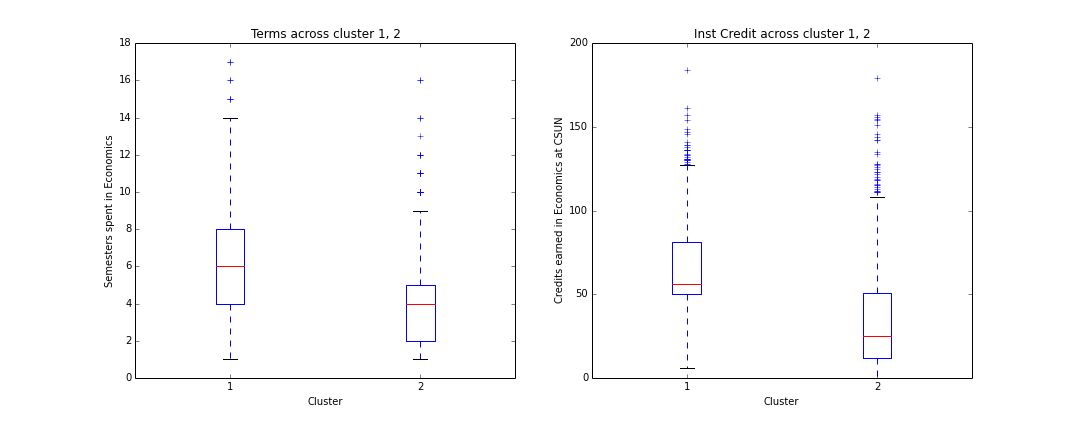
\includegraphics[width=0.4\columnwidth]{figures/box-Economics.png}
   \\
   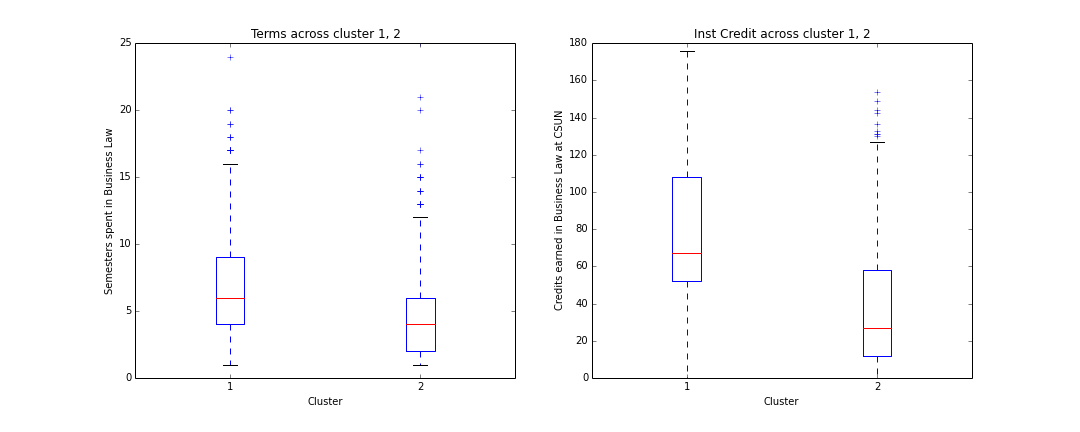
\includegraphics[width=0.4\columnwidth]{figures/box-Business-Law.png}
   \\
   \hline
   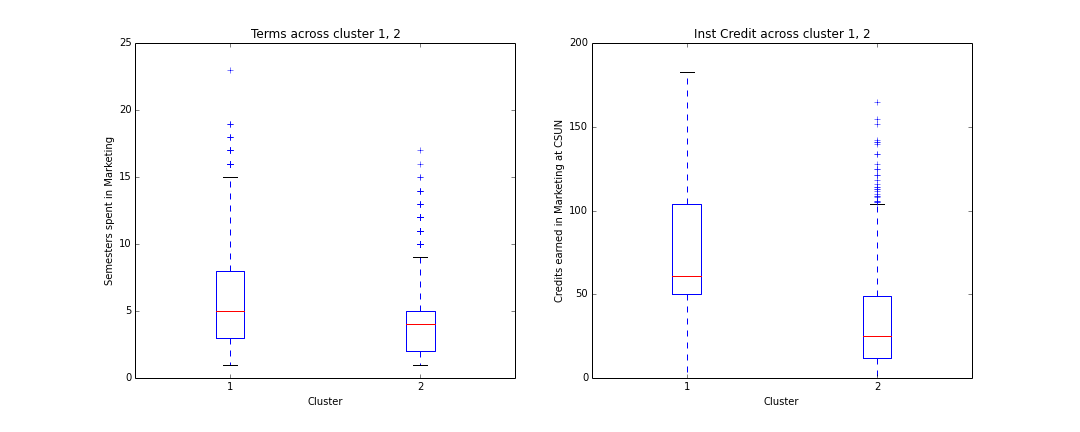
\includegraphics[width=0.4\columnwidth]{figures/box-marketing.png}
	\\  
   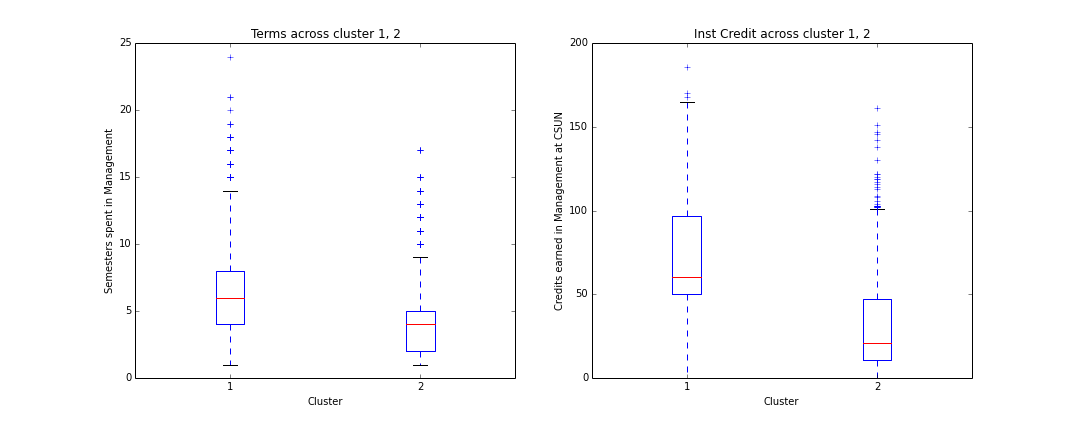
\includegraphics[width=0.4\columnwidth]{figures/box-management.png}
   \\
   \hline
   \end{tabular}
 \end{center}
  \caption{Time and units spent in each major}~\label{tab:boxplotTable}
\end{table}

\section{DISCUSSION}

Cluster analysis can also help to identify common traits among students within each cluster. For each department the second cluster spends on average four semesters enrolled with that major declared (\ref{tab:boxplotTable}). However the probability of these students graduating with the major is quite low (see \ref{tab:scoresTable}).
Note that precision in this case is equal to a student’s probability of graduating given that they are in cluster 1, and the false omission rate is equal to a student’s probability of graduating given that they are in cluster 2.




Principal component analysis (PCA) plots were used to investigate course contribution to cluster variation for each major. The PCA plots (\ref{tab:pcaTable}) determine the orthonormal directions of maximum variance in each dataset. The student grades are projected onto the first and second principal components, and the red and blue colors mark the clusters as determined by the K-Means algorithm. The management and marketing majors show more spatially separated clusters than those of economics and business law. 

A few course vectors are also shown; and here we see that, across majors, the ENGL205 and SOM120 vectors lie parallel  to the axis of separation between the two clusters, so these courses do not contribute meaningfully to cluster separation. Conversely, the class vectors (such as ACCT230) that lie perpendicular to the axis of separation contribute the most to cluster separation. Interestingly, there are courses (such as MATH150A) that play this role amongst several different majors. While these courses may not raise flags in any particular department, the fact that they are disproportionately driving student attrition rates should be of concern. We suggest that reforming, or at the very least investigating, these ‘hidden bottleneck’ courses may be crucial to understanding student attrition at large.



\section{LIMITATIONS AND FUTURE WORK}


Students may fail to graduate in CoBaE because they either change majors or discontinue their education at CSUN.  Hierarchical clustering methods could provide more detailed information on student outcomes, such as predicting which department a student might change their major to. Collaborative filtering methods could also give departmental recommendations to students considering a change of major. These methods could be used to develop early warning and recommendation systems for automated advisement, which would be especially beneficial to over-taxed advisement systems at comprehensive state universities such as CSUN.

Our results can be further refined by adding student metadata, for example: college year the major was declared, number of transfer credits, number of classes per term, financial aid, student demographics (such as age, gender, ethnicity, zip code) and various measures of student preparedness like SAT scores. With a more detailed feature space, our methods might be able to identify patterns and more well defined clusters. 

\section{CONCLUSION}

We trained unsupervised classifiers on grade data from four undergraduate majors at CSUN. In each case we found strongly predictive clusters, and found that cluster separation was driven disproportionately by a small number of bottleneck courses. We also found that training classifiers on the first three classes on the graduation pathway was an effective early detection method. We argue that reforming, or at the very least investigating, these bottleneck courses are crucial to understanding student attrition.
\begin{table}[h!]
 \begin{center}
   \begin{tabular}{| c | c |}
   \hline
   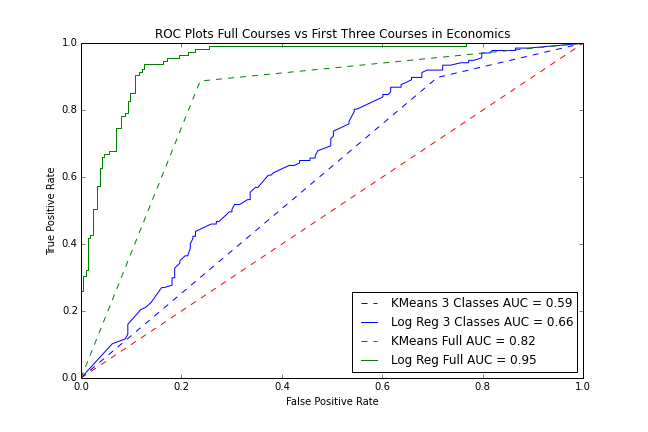
\includegraphics[width=0.2\textwidth]{figures/ROC-Economics.png}
   &
   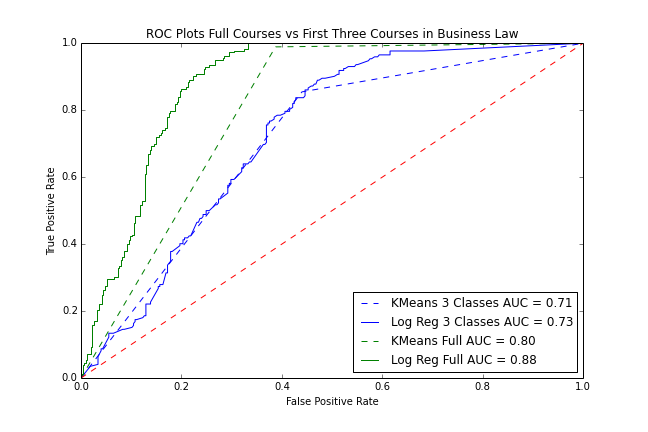
\includegraphics[width=0.2\textwidth]{figures/ROC-Business-Law.png}
   \\
   \hline
   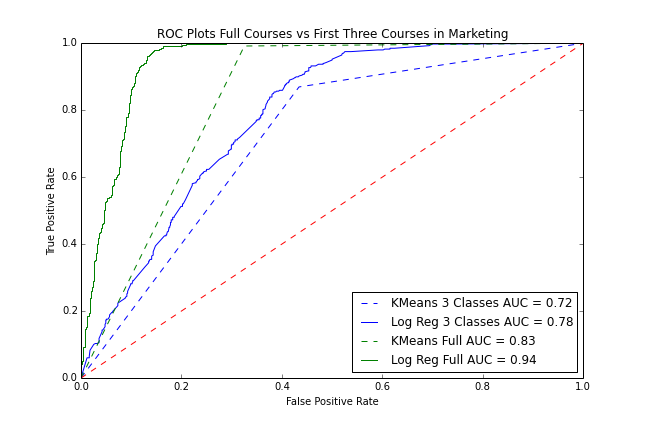
\includegraphics[width=0.2\textwidth]{figures/roc-marketing.png}
	&   
   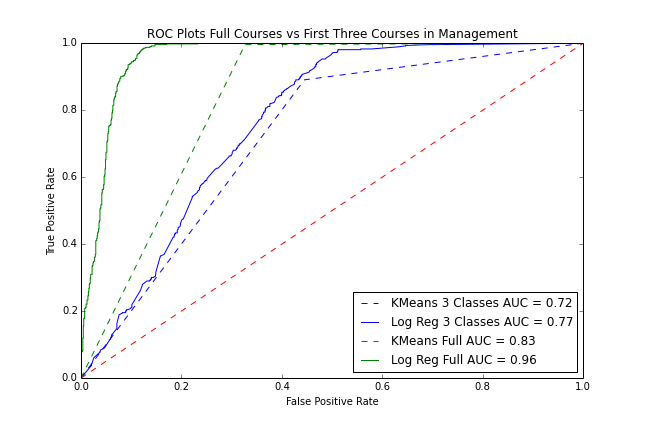
\includegraphics[width=0.2\textwidth]{figures/roc-management.png}
   \\
   \hline
   \end{tabular}
 \end{center}
 \caption{ROC plots for both classifiers on the full course set and the first three courses }~\label{tab:rocTable}
\end{table}


\begin{table}[h!]
 \begin{center}
   \begin{tabular}{| c | c |}

   \hline
   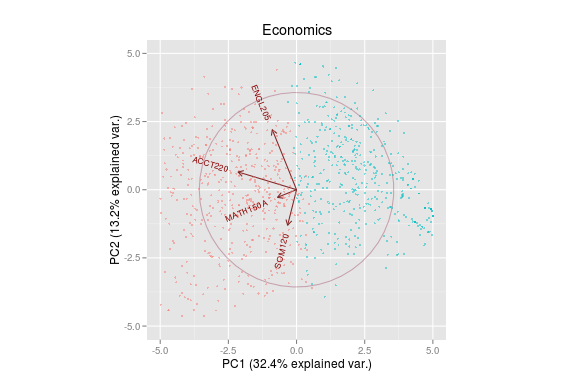
\includegraphics[width=0.2\textwidth]{figures/EconomicsPCA.png}
   &
   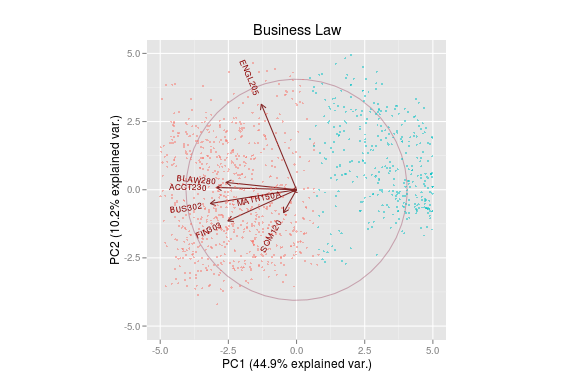
\includegraphics[width=0.2\textwidth]{figures/BusinessLawPCA.png}
   \\
   \hline
   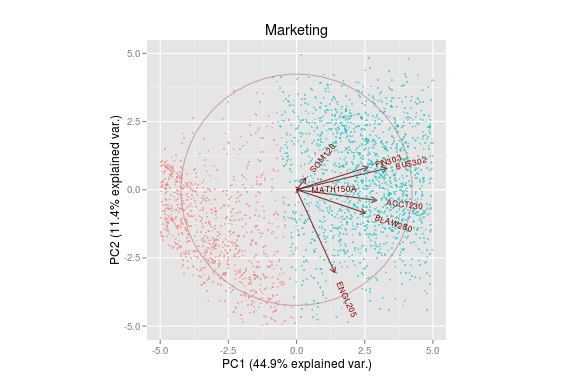
\includegraphics[width=0.2\textwidth]{figures/MarketingPCA.png}
	&   
   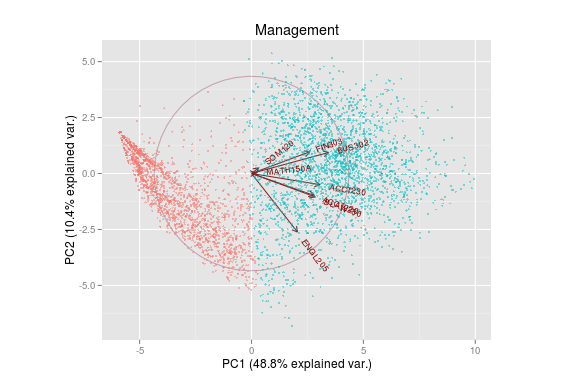
\includegraphics[width=0.2\textwidth]{figures/ManagementPCA.png}
   \\
   \hline
   \end{tabular}
 \end{center}
 \caption{PCA plots with course vector labels}~\label{tab:pcaTable}
\end{table}

\section{ACKNOWLEDGMENTS}

We gratefully acknowledge support from CSUN’s Office of the Provost and Academic Affairs. We thank Provost Harry Hellenbrand and VIce-Provost Michael Neubauer for their institutional support, and Bettina Huber, CSUN Director of Institutional Research, for making the data available. We also thank Yauheniya (Gina) Lahoda and Dr. Bruce Shapiro for numerous conversations during the Spring 2015 Machine Learning seminar. 



\balance{}
\bibliographystyle{SIGCHI-Reference-Format}
\bibliography{sample}

\end{document}
